\section{Introduction}
Memory is fundamental to intelligent agent, enabling the assimilation of prior experiences, contextual cues, and task-specific knowledge that underpin robust reasoning and decision-making ~\citep{wang2024towards,behrouz2024titans,du2025rethinking,zhang2024surveymemorymechanismlarge}.
While Large Language Models (LLMs)~\citep{deepseekr1,gpt4} demonstrate remarkable capabilities across a wide range of tasks, they exhibit significant limitations when engaged in long-context or multi-turn interaction scenarios due to fixed context windows and the ``lost in the middle'' problem~\citep{LostinMiddle}.
Memory systems are pivotal for overcoming these limitations, as they allow LLMs to maintain a persistent state across extended interactions.
Recent works~\citep{Li2025MemOSAO,memory3,Chhikara2025Mem0BP,Kang2025MemoryOO} address this challenge by building explicit external memory through sequential summarization and long term storage, enabling models to retain and retrieve relevant information over long horizons.

Note that a typical LLM memory system processes raw interaction data into manageable chunks, such as turn- or session-level in dialogue scenarios~\citep{Xu2025AMEMAM, li2025helloagainllmpoweredpersonalized}, organizes them into long-term memory (e.g., databases or knowledge graphs) by indexing them into memory units, and continuously updates by adding new information and discarding outdated or conflicting content~\citep{DBLP:conf/aaai/ZhongGGYW24}. 
This enables retrieval of relevant memories, improving coherence, and personalization in long-context, multi-turn scenarios.


\textbf{Challenges.} 
Despite these advances, as shown in Figure \ref{fig:motivation}, contemporary memory systems still suffer from significant inefficiencies and consistency issues. 
First, in long interactions (e.g., dialogue scenarios), both user inputs and model responses often contain substantial redundant information~\citep{maharana2024evaluatinglongtermconversationalmemory, DBLP:conf/iclr/WuWYZCY25}. Such information is typically irrelevant to downstream tasks or subsequent memory construction, and in some cases, may even negatively affect the model’s in-context learning capability~\citep{liu2023lostmiddlelanguagemodels, DBLP:conf/iclr/PanWJLCL0LZQ025}. However, current mainstream memory-related studies generally process the raw information directly without any filtering or refinement, leading to high overhead from noisy or irrelevant data. 
This inflates token consumption  without proportional gains in reasoning quality or coherence. 
Second, memory construction typically \textbf{treats each turn in isolation or relies on rigid context-window boundaries}, failing to model semantic connections across different turns~\citep{tan2025prospectretrospectreflectivememory}.
% As a result, stored memories can become either overly generic or excessively granular, triggering redundant or ineffective recall that wastes precious input length.
As a result, during subsequent memory item construction, the backbone LLM may generate inaccurate or incomplete item representations due to overly entangled topics or semantics, leading to the loss of crucial contextual details.
Third, memory updates and forgetting are usually performed directly \textbf{during inference and task execution}. 
This tight coupling introduces long test-time latency in long-horizon tasks and prevents deeper, reflective processing of past experiences.

% In contrast, human memory offers a compelling model of efficiency and adaptability~\citep{liu2025advances}. 
% It operates through a hierarchical architecture: sensory memory pre-filters incoming stimuli before they reach short-term memory, which actively integrates, manipulates, and reasons over task-relevant content. 
% Over time, salient information is selectively consolidated into long-term memory processing in sleep time. 
% This dynamic, multi-stage system balances retention, compression, and retrieval, striking an optimal trade-off between performance and resource usage.

% In contrast, human memory efficiently processes information through a hierarchical system: sensory memory pre-filters stimuli, short-term memory actively integrates and reasons over relevant content, and long-term memory selectively consolidates salient information in sleep time.


\begin{wrapfigure}{r}{0.6\columnwidth}
    \vspace{-0.4cm}
    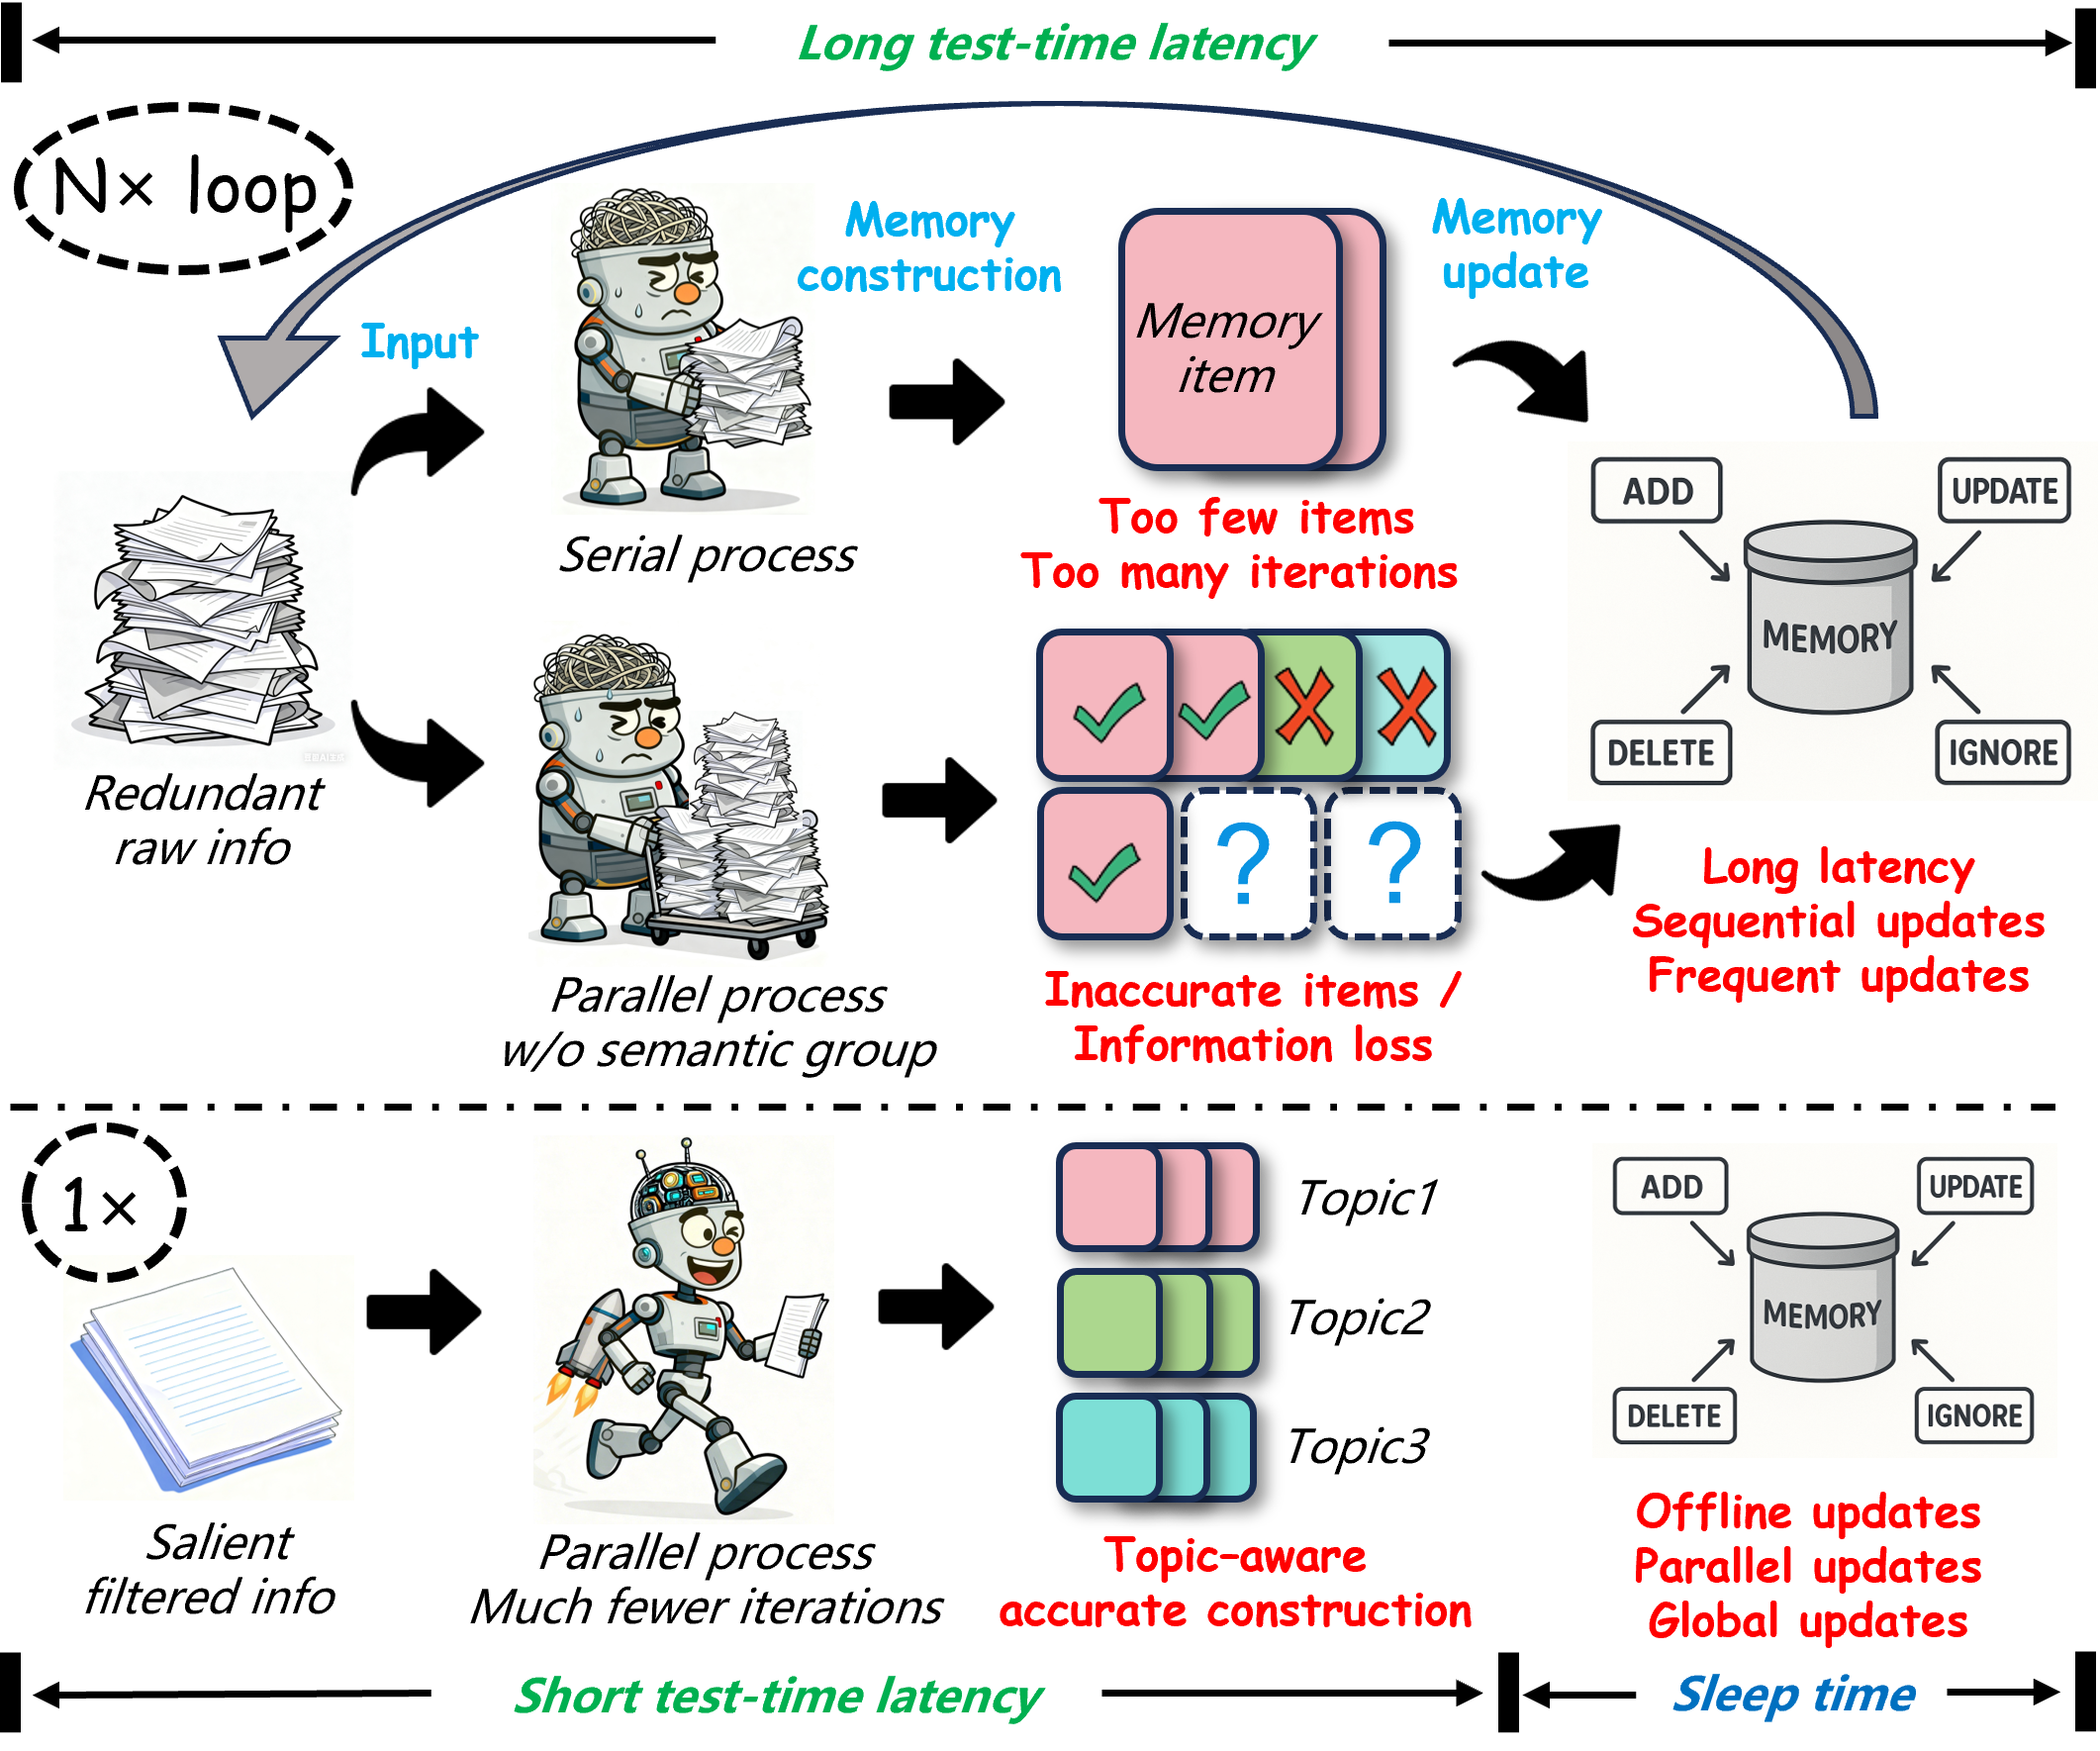
\includegraphics[width=1.0\linewidth]{figure/motivation.png}
    \vspace{-0.5cm}
    \caption{\change{Comparison of previous works and \textbf{LightMem}.}}
    \label{fig:motivation}
    \vspace{-0.2cm}
\end{wrapfigure}

\textbf{Building Lightweight Memory.} 
%To build robust and scalable LLM agents, lightweight memory systems are essential, particularly for long-horizon dialogue and sustained human–agent interaction.
Inspired by the efficiency and structure of human memory, we introduce \textbf{LightMem}.
In particular, LightMem emulates human memory through three key components: 
(1) A \textit{pre-compression sensory memory module} that filters redundant or low-value tokens from raw input and buffers the distilled content. 
(2) A \textit{topic-aware short-term memory} that leverages semantic and topical similarity to dynamically group related utterances into coherent segments.
By adaptively determining segment boundaries based on content instead of fixed window sizes, this module produces more concentrated and meaningful memory units. 
This not only reduces the frequency of memory construction but also enables more precise and efficient retrieval during inference.
(3) A \textit{sleep-time update} mechanism for long-term memory maintenance. 
New memory entries are initially stored with timestamps to support immediate (``soft'') updates for real-time responsiveness. 
Later, during designated offline periods (i.e., ``sleep''), the system reorganizes, de-duplicates, and abstracts these entries, resolving inconsistencies and strengthening cross-knowledge connections. 
Crucially, this decouples expensive memory maintenance from real-time inference, enabling reflective, high-fidelity updates without introducing latency. 
By systematically filtering, organizing, and consolidating relevant information, LightMem substantially reduces computational overhead and API costs while sustaining accurate, coherent reasoning over extended interactions.
We detail each component in \S\ref{sec:method}. 

\textbf{Results and Evaluation.}
% On LongMemEval~\citep{DBLP:conf/iclr/WuWYZCY25}, LightMem outperforms the strongest baseline by 2.70\%--9.65\% in QA accuracy while achieving significant efficiency gains: reducing token usage by 32$\times$--117$\times$, API calls by 17$\times$--177$\times$, and runtime by 1.67$\times$--12.45$\times$ across GPT and Qwen backbones. These advantages are maintained after offline updates.
% Furthermore, case studies in \S\ref{sec:case_study} reveal that the offline ``sleep-time'' consolidation enables more reliable long-term knowledge updates,  mitigating information loss and inconsistency in extended interactions.
%Together, these results demonstrate that a human-inspired memory architecture, grounded in filtering, structured organization, and asynchronous sleep-time consolidation, can enable AI that are not only scalable and efficient but also coherent and contextually robust over long horizons.
% On LongMemEval~\citep{DBLP:conf/iclr/WuWYZCY25}, LightMem achieves consistently higher QA accuracy than the strongest baseline (up to 9.65\% with GPT and 7.67\% with Qwen) while substantially improving efficiency—reducing token usage by up to 117$\times$, API calls by up to 177$\times$, and runtime by up to 12.45$\times$ across both backbones.
% On the LoCoMo benchmark~\citep{maharana2024evaluatinglongtermconversationalmemory}, LightMem maintains these advantages, achieving 6.10\%--29.29\% higher accuracy along with large efficiency gains, improving token usage by up to 20.92$\times$, reducing API calls by up to 55.48$\times$, and accelerating runtime by up to 8.21$\times$ across GPT and Qwen backbones.
% Furthermore, case studies in \S\ref{sec:case_study} show that the offline sleep-time consolidation further enhances long-term memory reliability, mitigating information loss.
\change{On LongMemEval~\citep{DBLP:conf/iclr/WuWYZCY25}, LightMem consistently outperforms the strongest baseline, improving accuracy by 2.09\%--6.40\% with GPT and up to 7.67\% with Qwen.
In terms of overall efficiency (online + offline), LightMem reduces total token usage by up to 38$\times$ for GPT and 21.8$\times$ for Qwen, lowers API calls by up to 30$\times$ and 17.1$\times$, and accelerates runtime by up to 12.4$\times$ and 6.3$\times$, respectively.
If considering only online test-time costs, the gains become even larger: LightMem cuts token usage by up to 105.9$\times$ (GPT) and 117.1$\times$ (Qwen), and reduces API calls by up to 159.4$\times$ and 309.9$\times$.
On the LoCoMo benchmark~\citep{maharana2024evaluatinglongtermconversationalmemory}, LightMem maintains strong advantages, achieving 6.10\%--29.29\% higher accuracy and substantial efficiency improvements—boosting token efficiency by up to 20.92$\times$, reducing API calls by up to 55.48$\times$, and speeding up runtime by up to 8.21$\times$ across GPT and Qwen backbones.}
Furthermore, case studies in \S\ref{sec:case_study} show that the offline “sleep-time’’ consolidation enhances long-term memory reliability, mitigating information loss.
